\documentclass[a4paper]{article}

\usepackage[utf8]{inputenc}  
\usepackage[francais]{babel}  
\usepackage[top=2cm, bottom=2cm, left=2cm, right=2cm]{geometry}
\usepackage{graphicx}

\begin{document}

\begin{titlepage}
	~ 
	\vfill
	\begin{center}
		\begin{Huge}
			Projet Administration Réseau : \\ Spécifications de l'architecture DNS et Tutorial de maintenance de l'installation\\
		\end{Huge}
	\vfill
		\textbf{Hexanôme 4211 :} 
			\\Sandra \bsc{Mondain}, Elisa \bsc{Abidh}, 
			\\Gaël \bsc{Motte}, Armand \bsc{Rossius}, 
			\\Nicolas \bsc{Silva}, Julien \bsc{Levesy}\\
	\vfill
	\end{center}
	\vfill
\end{titlepage}

\newpage
\tableofcontents
\newpage

\section{Spécification de l'architecture DNS}

\subsection{Politique de nommage et déploiement des services d'annuaires machines }



\subsection{Configuration de base des serveurs DHCP}

\subsubsection{Site Lyon : AIP Bat Jacquard }

\paragraph{Plages IP addressables :} 
\begin{itemize}
\item[10.1.1.2 à 10.1.1.253] Plages postes
\item[10.1.2.2 à 10.1.2.253] Plages Automates
\end{itemize}


\paragraph{Plages IP d'exclusion :}
\begin{itemize}
\item[10.1.0.2 à 10.1.0.253] : Plage réservée au déploiement de serveurs architecturaux et services
\end{itemize}

\paragraph{Configuration du serveur DHCP}

\subparagraph{Configuration serveur}
\begin{itemize}
\item[Adresse réseau]: 10.1.0.2
\item[Masque de sous réseau]: 255.255.254.0
\item[Adresse DNS]: 10.1.0.3
\end{itemize}

\subparagraph{Sous Réseau salles}
\begin{itemize}
\item[Adresse réseau]: 10.1.1.0
\item[Adresse broadcast]: 10.1.1.255
\item[Masque de sous réseau]: 255.255.255.0
\item[Durée du Bail Long]: 87\% du temps utile
\item[Durée du Bail court]: 50\% du tempsutie
\item[Routeur (passerelle)]: 10.1.1.1
\item[Adresse DNS]: 10.1.0.3
\end{itemize}

\subparagraph{Sous réseau automates}
\begin{itemize}
\item[Adresse réseau]: 10.1.2.0
\item[Adresse broadcast]: 10.1.2.255
\item[Masque de sous réseau]: 255.255.255.0
\item[Durée du Bail Long]: 87\% du temps utile
\item[Durée du Bail court]: 50\% du tempsutie
\item[Routeur (passerelle)]: 10.1.2.1
\item[Adresse DNS]: 10.1.0.3
\end{itemize}

\subsubsection{Site Lyon : AIP Bat Ferrié}

\paragraph{Plages IP adressables :} 
\begin{itemize}
\item[10.2.1.2 à 10.2.1.253]
\item[10.2.2.2 à 10.2.2.253]
\end{itemize}

\paragraph{Plages IP d'exclusion :}
\begin{itemize}
\item[10.2.0.2 à 10.2.0.253] : Plage réservée au déploiement de serveurs architecturaux et services
\end{itemize}

\paragraph{Configuration du serveur DHCP}

\begin{itemize}
\item[Adresse réseau]: 10.2.0.2
\item[Masque de sous réseau]: 255.255.255.0
\item[Adresse DNS]: 10.2.0.3
\end{itemize}

\subparagraph{Sous Réseau salles}
\begin{itemize}
\item[Adresse réseau]: 10.2.1.0
\item[Adresse broadcast]: 10.2.1.255
\item[Masque de sous réseau]: 255.255.255.0
\item[Durée du Bail Long]: 87\% du temps utile
\item[Durée du Bail court]: 50\% du tempsutie
\item[Routeur (passerelle)]: 10.2.1.1
\item[Adresse DNS]: 10.2.0.3
\end{itemize}

\subparagraph{Sous réseau automates}
\begin{itemize}
\item[Adresse réseau]: 10.2.2.0
\item[Adresse broadcast]: 10.2.2.255
\item[Masque de sous réseau]: 255.255.255.0
\item[Durée du Bail Long]: 87\% du temps utile
\item[Durée du Bail court]: 50\% du tempsutie
\item[Routeur (passerelle)]: 10.2.2.1
\item[Adresse DNS]: 10.2.0.3
\end{itemize}

\subsubsection{Site Roanne : IUT}

\paragraph{Plages IP addressables :} 
\begin{itemize}
\item[10.3.1.2 à 10.3.1.253]
\item[10.3.2.2 à 10.3.2.253]
\end{itemize}

\paragraph{Plages IP d'exclusion :}
\begin{itemize}
\item[10.3.0.2 à 10.3.0.253] : Plage réservée au déploiement de serveurs architecturaux et services
\end{itemize}

\paragraph{Configuration du serveur DHCP}

\begin{itemize}
\item[Adresse réseau]: 10.3.0.2
\item[Masque de sous réseau]:255.255.254.0
\item[Adresse DNS]: 10.3.0.3
\end{itemize}

\subparagraph{Sous Réseau salles}
\begin{itemize}
\item[Adresse réseau]: 10.3.1.0
\item[Adresse broadcast]: 10.3.1.255
\item[Masque de sous réseau]: 255.255.255.0
\item[Durée du Bail Long]: 87\% du temps utile
\item[Durée du Bail court]: 50\% du tempsutie
\item[Routeur (passerelle)]: 10.3.1.1
\item[Adresse DNS]: 10.3.0.3
\end{itemize}

\subparagraph{Sous réseau automates}
\begin{itemize}
\item[Adresse réseau]: 10.3.2.0
\item[Adresse broadcast]: 10.3.2.255
\item[Masque de sous réseau]: 255.255.255.0
\item[Durée du Bail Long]: 87\% du temps utile
\item[Durée du Bail court]: 50\% du tempsutie
\item[Routeur (passerelle)]: 10.3.2.1
\item[Adresse DNS]: 10.3.0.3
\end{itemize}

\subsection{Politique d'affectation d'IP par site}

Chaque site est équipé de deux sous réseaux, l'un destiné aux postes de types PC destinés au cours et l'autre destiné à l'affectation d'automates. Un problème se pose donc au niveau du DHCP quant à l'affectation dans tel où tel sous réseau de la machine ayant émis la requête.\\
Nous faisons donc l'hypothèse, en accord avec l'équipe enseignante, que les automates possèdent chacun un fichier de configuration éditable par les administrateurs, contenant l'adresse fixée (dans le sous réseau automates du site) souhaitée et le nom DNS cohérent, qui seront transmises dans la trame DHCPREQUEST.\\
Ainsi si l'IP est disponible ( assertion au préalable vérifiée par le serveur DHCP :=) ) elle sera affectée dans un bail soumis à la machine demande, comme spécifié dans le fonctionnement du DHCP.\\
Dans le cas contraire, l'affectation est refusée et l'automate procédera à des demandes à intervalle régulier jusqu'à ce qu'il obtienne ce qu'il désire.\\
Notons bien que la plage d'adressage des sous réseaux automates est différente en fonction du site, ainsi en cas de déplacement il sera obligatoire de recréer un fichier de configuration par site avant la première connexion du dispositif. 

\subsection{Gestion d'annuaires utilisateur LDAP}

Afin de garantir une qualité de service et une utilisabilté même si le site de Lyon-Jacquard est injoignable par réseau, nous décidons d'appliquer une politique de réplication d'un groupe LDAP d'utilisateurs autorisés à utiliser les équipements de l'AIP, sur les trois annuaires LDAP actuellement en fonction sur les campus équipés d'installations AIP.

\section{Tutoriel de maintenance}

\subsection{Principes d'organisation du réseau par site}

\subsubsection{Site Lyon Jacquard}

\begin{center}
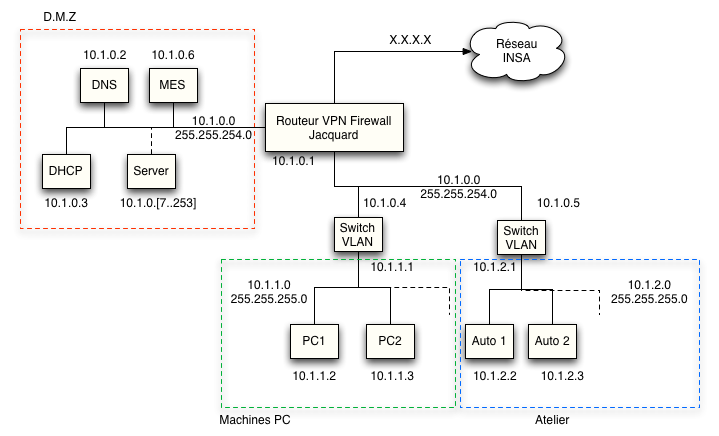
\includegraphics[scale=0.6]{SiteJacquard.png}
\end{center}

\subsubsection{Site Lyon Ferrié}

\begin{center}
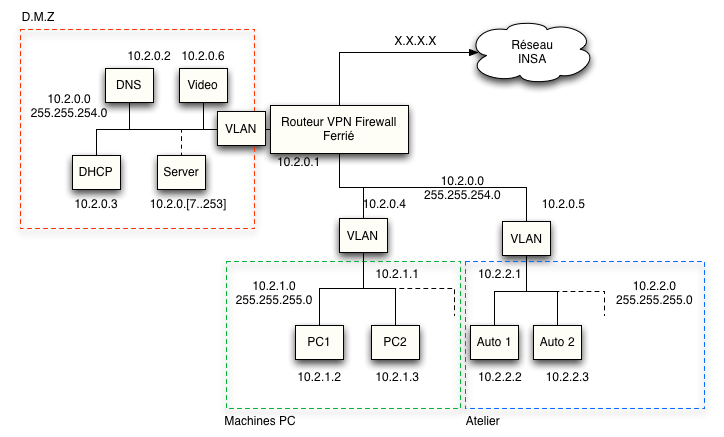
\includegraphics[scale=0.6]{SiteFerrie.png}
\end{center}

\subsubsection{Site Roanne}

\begin{center}
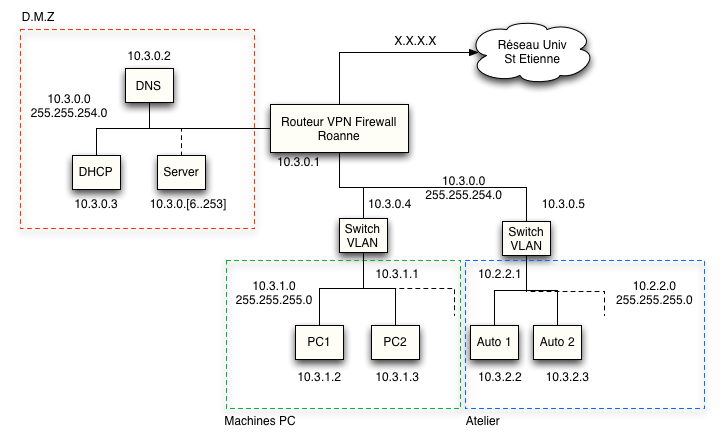
\includegraphics[scale=0.6]{SiteRoanne.png}
\end{center}

\subsection{Comment ajouter une machine type P.C sur le réseau ?}

\subsubsection{Restauration d'une configuration standard sur le poste}

\subsubsection{Création d'une entrée dans l'annuaire DNS}

\subsubsection{Création d'une entrée dans l'annuaire LDAP du campus}

\subsubsection{Bind de la machine au LDAP du campus}

\subsubsection{Opérations de vérification}

\subsection{Comment supprimer une machine type P.C sur le réseau ?}

\subsubsection{Suppression de l'entrée LDAP de la machine}

\subsubsection{Suppression de l'entrée DNS de la machine}

\subsubsection{Opérations de vérification}

\subsection{Comment déplacer une plateforme de TP temporairement ?}

\subsubsection{Sur le site de départ}

\subsubsection{Sur le site de déplacement}

\subsection{Comment ajouter une plateforme de TP  ?}

\subsubsection{Création de l'entrée DNS}

\subsection{Comment supprimer une plateforme de TP définitivement ?}

\subsubsection{Suppression de l'entrée DNS}

\end{document}